\documentclass[11pt]{article}
\usepackage{mathtools}
\usepackage{amssymb}
\usepackage{amsthm}
\usepackage{polski}
\usepackage[utf8]{inputenc}
\usepackage{geometry}
\usepackage{mnsymbol}
\usepackage{graphicx}
\usepackage{textgreek}
\usepackage{float}
\usepackage{caption}
\author{Łukasz Jezapkowicz}
\title{Wzmacniacz operacyjny}
\date{23.05.2019}
\begin{document}
\newgeometry{tmargin=2cm,bmargin=2cm,lmargin=2cm,rmargin=2cm}
\maketitle
\tableofcontents \newpage
\section{Wzmacniacz operacyjny w układzie wzmacniacza odwracającego}
\subsection{Cel ćwiczenia}
Celem ćwiczenia było zapoznanie się z prostym układem wzmacniacza operacyjnego w układzie wzmacniacza odwracającego oraz wyznaczenie oporu i wzmocnienia napięciowego przy pomocy analizy Transient.
\subsection{Przebieg ćwiczenia}
Na pulpicie symulacyjnym zbudowałem układ wzmacniacza operacyjnego w układzie wzmacniacza odwracającego widoczny na \textbf{Rys. 1}. Układ zawiera dwa źródła napięcia stałego $V_1=15V$,$V_2=15V$, rezystor $R_1=10k\Omega$, wzmacniacz operacyjny $LF356N$ oraz rezystor $R_2$, którego wartość 
należało wyznaczyć tak, żeby wzmocnienie napięciowe $k_u=-10$. Jest to układ wzmacniacza odwracającego więc jego wzmocnienie napięciowe możemy obliczyć z wzoru $k_u=\frac{-R_2}{R_1}$. Po wyznaczeniu z tego równania $R_2$ i podstawieniu odpowiednich wartości dostajemy $R_2=100k\Omega$.
Do układu podłączyłem również generator $XFG1$, o częstotliwości $1kHz$ i amplitudzie $10mV$, oraz oscyloskop $XSC1$, które pomogły mi obserwować przebieg napięcia wejściowego i wyjściowego.
\begin{figure}[H]
\centering
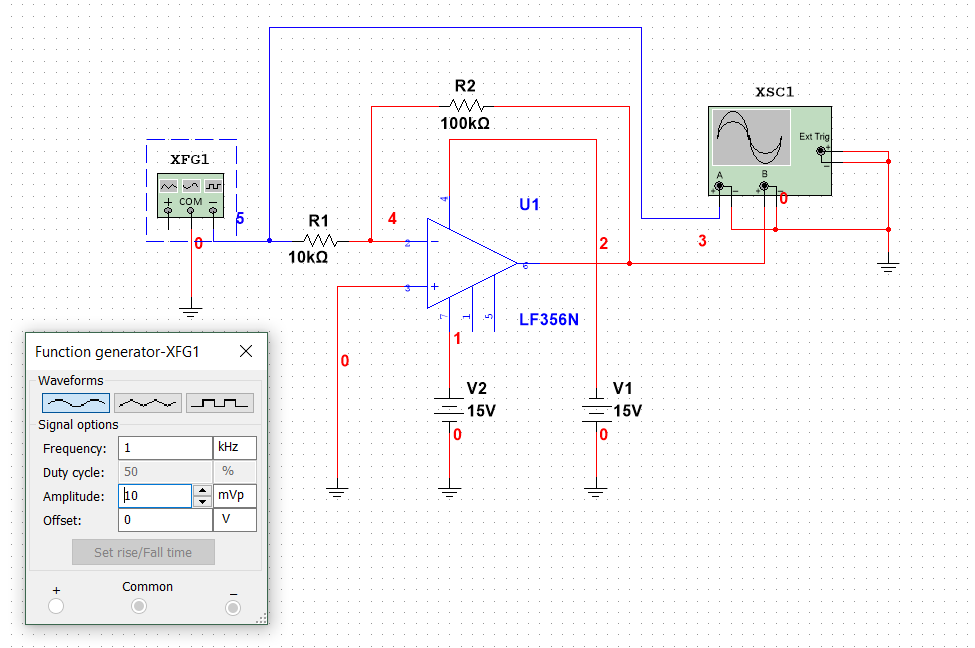
\includegraphics[width=10cm]{1}
\caption*{\textbf{Rys. 1}: Schemat układu wzmacniacza operacyjnego w układzie wzmacniacza odwracającego, dla którego $k_u=-10$}
\end{figure}
\noindent Celem zadania było wyznaczenie wzmocnienia napięciowego przy pomocy analizy Transient. Na \textbf{Rys. 2} i \textbf{Rys. 3} widać odpowiednio ekran oscyloskopu oraz wyniki pomiarów analizy Transient. Na oscyloskopie wybrałem tryb AC by oba przebiegi były symetryczne. Łatwo zauważyć, że sygnał wyjściowy
jest odwrócony.Do policzenia wzmocnienia napięciowego
użyjemy wzoru $k_u=\frac{{\Delta}U_{Wy}}{{\Delta}U_{We}}$. W celu łatwych obliczeń policzę iloraz podwojonych amplitud sygnałów (dy). Z analizy Transient mam: $k_u=\frac{-199.9350mV}{19.9945mV}=-9.999$ zaś z obrazu oscyloskopu $k_u=\frac{-199.631mV}{19.964mV}=-9.999$. Wyniki są zatem zgodne.
\begin{figure}[H]
\centering
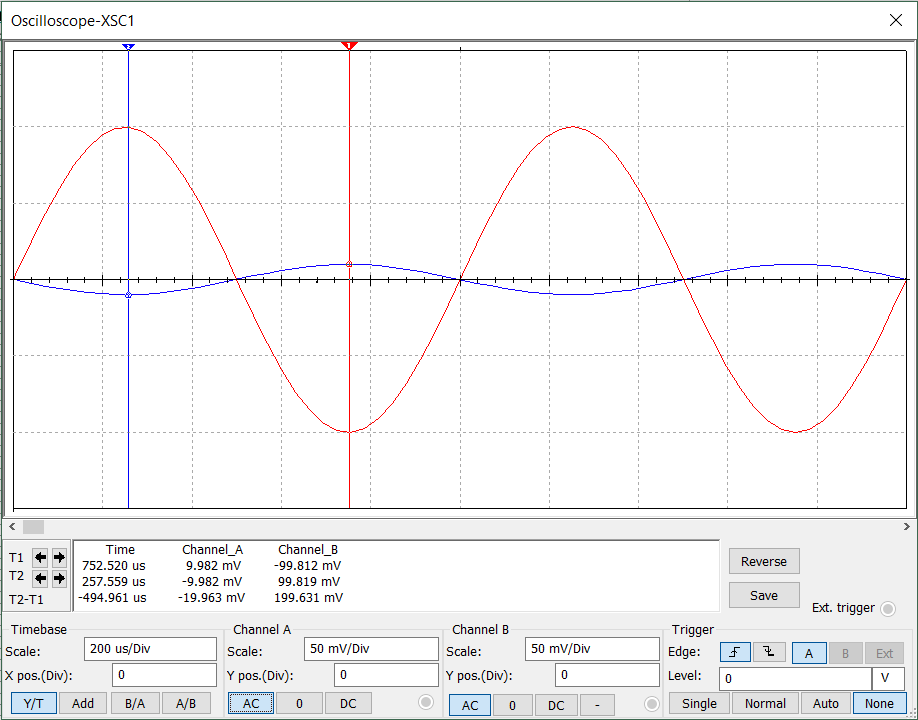
\includegraphics[width=10cm]{2}
\caption*{\textbf{Rys. 2}: Ekran oscyloskopu dla układu wzmacniacza widocznego na Rys. 1, gdzie $k_u=-10$}
\end{figure}
\begin{figure}[H]
\centering
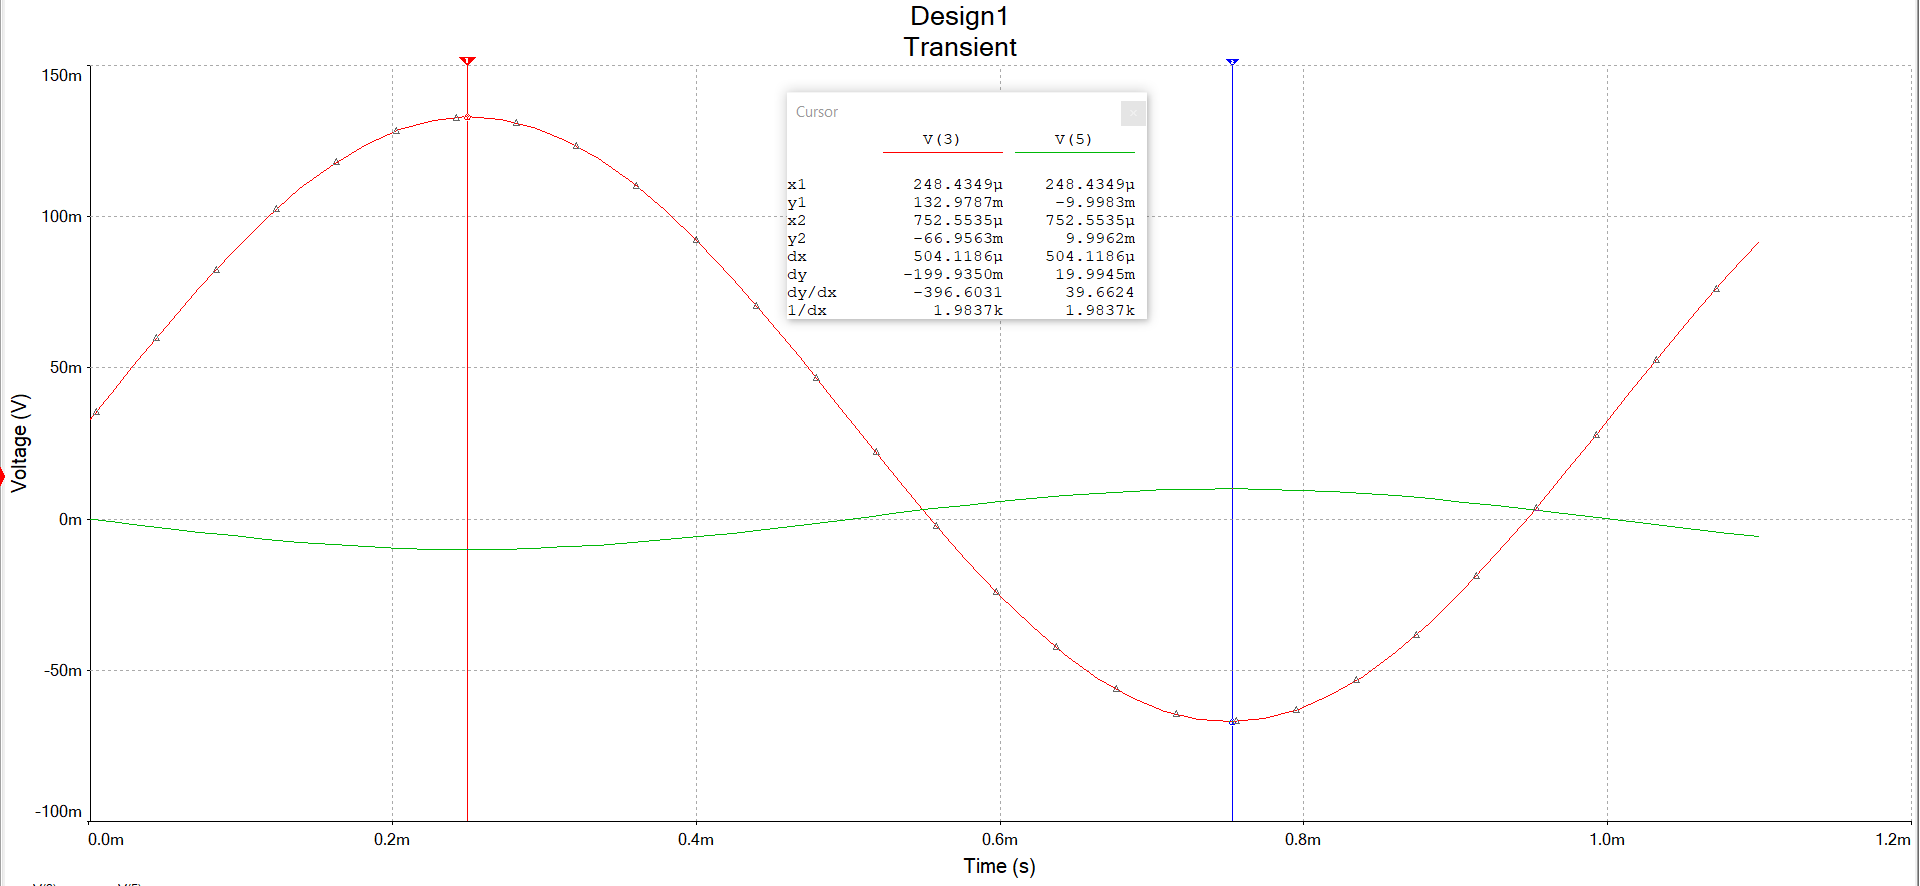
\includegraphics[width=10cm]{3}
\caption*{\textbf{Rys. 3}: Analiza Transient dla układu wzmacniacza widocznego na Rys. 1, gdzie $k_u=-10$ }
\end{figure}
\subsection{Wnioski}
Wykonane ćwiczenie pokazuje, że wzór na wzmocnienia napięciowe $k_u=\frac{-R_2}{R_1}$ jest poprawny i daje praktycznie dokładną wartość wzmocnienia napięciowego co udowodniłem obliczając wzmocnienie napięciowe przy pomocy ekranu oscyloskopu i analizy Transient przy pomocy wzoru  $k_u=\frac{{\Delta}U_{Wy}}{{\Delta}U_{We}}$. W ćwiczeniu zauważyliśmy również odwrócony sygnał wyjściowy.
\section{Wzmacniacz operacyjny odwracający w układzie sumatora}
\subsection{Cel ćwiczenia}
Celem ćwiczenia było zapoznanie się z układem wzmacniacza operacyjnego odwracającego w układzie sumatora oraz bliższe przyjrzenie się przebiegom wejściowym i przebiegowi wyjściowemu.
\subsection{Przebieg ćwiczenia}
Układ sumatora to układ, w którym na wejściu podane jest kilka napięć, które sumują się przed spotkaniem z wzmacniaczem odwracającym. Na pulpicie symulacyjnym zbudowałem układ wzmacniacza operacyjnego odwracającego w układzie sumatora widoczny na \textbf{Rys. 4}. Układ zawiera dwa źródła napięcia stałego $V_1=15V$,$V_2=15V$, trzy rezystory $R_1=10k\Omega$,$R_2=100k\Omega$,$R_3=10k\Omega$ oraz wzmacniacz operacyjny $LF356N$.
Do układu podłączyłem również generatory $XFG1$ oraz $XFG2$, na które podałem odpowiednio sygnał prostokątny o częstotliwości $100Hz$, wypełnieniu $50\%$ i amplitudzie $1V$ oraz sygnał zmienny o częstotliwości $2kHz$ i amplitudzie $500mV$. Podłączyłem również oscyloskop $XSC1$. Ponieważ podaje na wejście dwa
sygnały więc $U_{We}=U_{We1}+U_{We2}$. Do obliczeń przyjmuję $R=R_1=R_3=10k\Omega$. Na wyjściu dostajemy $U_{Wy}=-U_{R2}=-I_{We}*R_2=-(I_{We1}+I_{We2}*R_2=-(\frac{U_{We1}}{R}+\frac{U_{We2}}{R})*R_2=-\frac{U_{We}}{R}*R_2$. Wzmocnienie napięciowe zatem jest równe: $k_u=-\frac{R_2}{R}=-10$.
\begin{figure}[H]
\centering
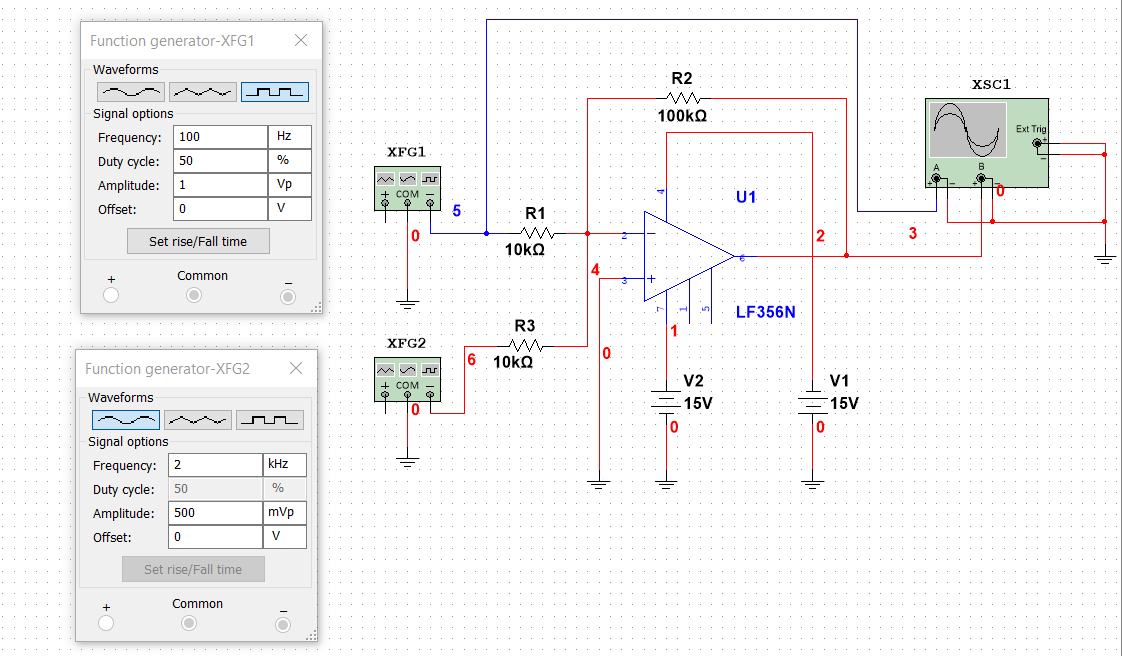
\includegraphics[width=10cm]{4}
\caption*{\textbf{Rys. 4}: Schemat układu wzmacniacza operacyjnego odwracającego w układzie sumatora, dla którego $k_u=-10$}
\end{figure}
\noindent Celem zadania było przyjrzenie się przebiegom sygnałów wejściowych oraz sygnału wyjściowego. Na \textbf{Rys. 5} i \textbf{Rys. 6} widać odpowiednio ekran oscyloskopu oraz wyniki analizy Transient dla układu z \textbf{Rys. 4}. Analiza Transient idealnie pokazuje efekt sumowania dwóch sygnałów wejściowych,
ich odwrócenia i wzmocnienia. 
\begin{figure}[H]
\centering
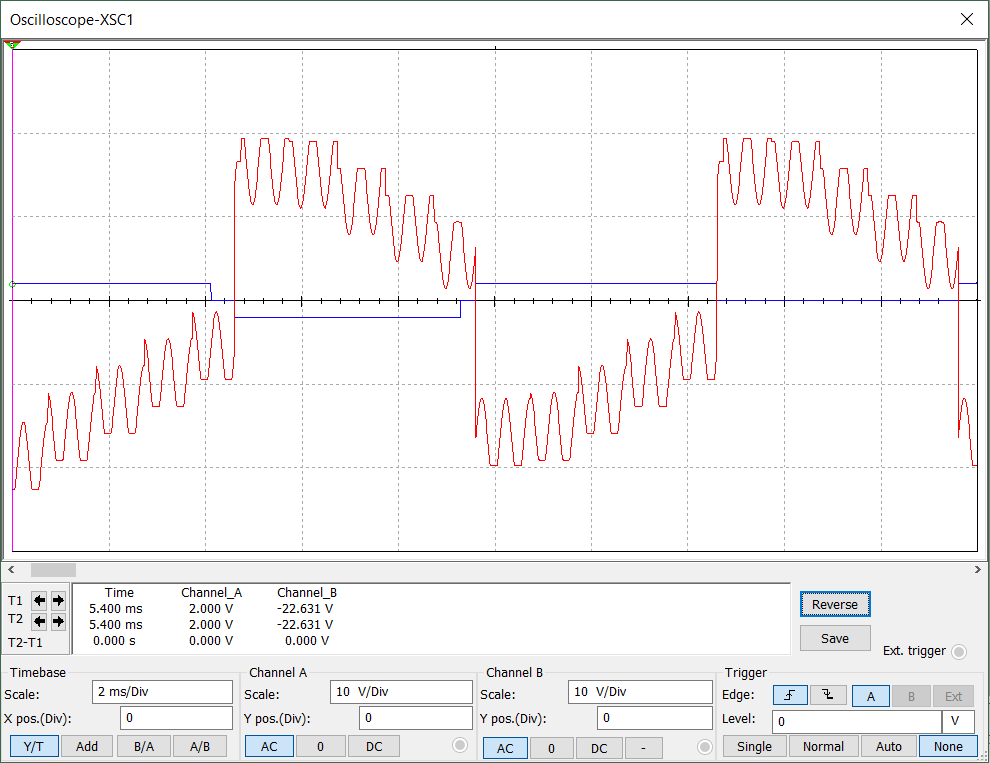
\includegraphics[width=10cm]{5}
\caption*{\textbf{Rys. 5}: Ekran oscyloskopu dla układu wzmacniacza widocznego na Rys. 4, gdzie $k_u=-10$. Widoczny jest tu sygnał wejściowy prostokątny}
\end{figure}
\begin{figure}[H]
\centering
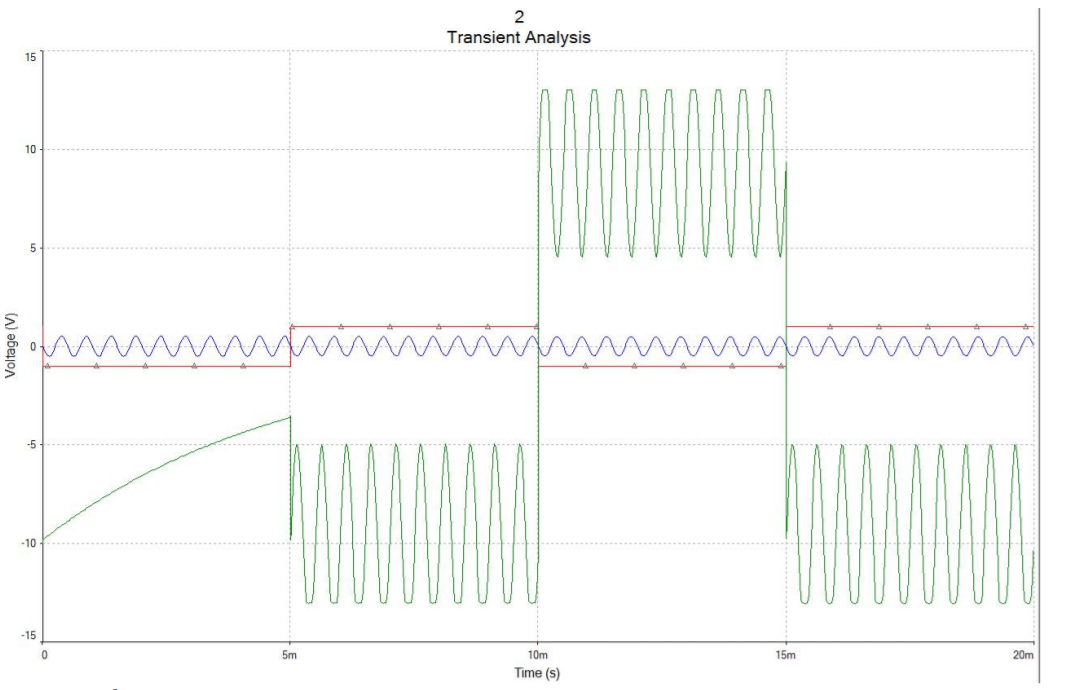
\includegraphics[width=10cm]{6_dozmiany}
\caption*{\textbf{Rys. 6}: Analiza Transient dla układu wzmacniacza widocznego na Rys. 4, gdzie $k_u=-10$. Sygnał wejściowy prostokątny jest zaznaczony kolorem czerwonym, zaś zmienny jest koloru niebieskiego. Przebieg wyjściowy jest zaznaczony kolorem zielonym. }
\end{figure}
\subsection{Wnioski}
Wykonane ćwiczenie pokazuje efekt nakładania się dwóch sygnałów wejściowych i przebieg końcowego sygnału wyjściowego po przejściu przez wzmacniacz operacyjny odwracający w układzie sumatora. Wyniki analizy Transient pokazały jak owy przebieg wygląda dla przykładowego obwodu z \textbf{Rys. 4}.
\section{Wzmacniacz operacyjny w układzie wzmacniacza nieodwracającego}
\subsection{Cel ćwiczenia}
Celem ćwiczenia było zapoznanie się z prostym układem wzmacniacza operacyjnego w układzie wzmacniacza nieodwracającego oraz wyznaczenie oporu i wzmocnienia napięciowego przy pomocy analizy Transient.
\subsection{Przebieg ćwiczenia}
Na pulpicie symulacyjnym zbudowałem układ wzmacniacza operacyjnego w układzie wzmacniacza nieodwracającego widoczny na \textbf{Rys. 7}. Układ zawiera dwa źródła napięcia stałego $V_1=15V$,$V_2=15V$, rezystor $R_1=10k\Omega$, wzmacniacz operacyjny $LF356N$ oraz rezystor $R_2$, którego wartość 
należało wyznaczyć tak, żeby wzmocnienie napięciowe $k_u=5$. Jest to układ wzmacniacza nieodwracającego więc jego wzmocnienie napięciowe możemy obliczyć z wzoru $k_u=\frac{R_1+R_2}{R_1}$. Po wyznaczeniu z tego równania $R_2$ i podstawieniu odpowiednich wartości dostajemy $R_2=40k\Omega$.
Do układu podłączyłem również generator $XFG1$, o częstotliwości $1kHz$ i amplitudzie $10mV$, oraz oscyloskop $XSC1$, które pomogły mi obserwować przebieg napięcia wejściowego i wyjściowego.
\begin{figure}[H]
\centering
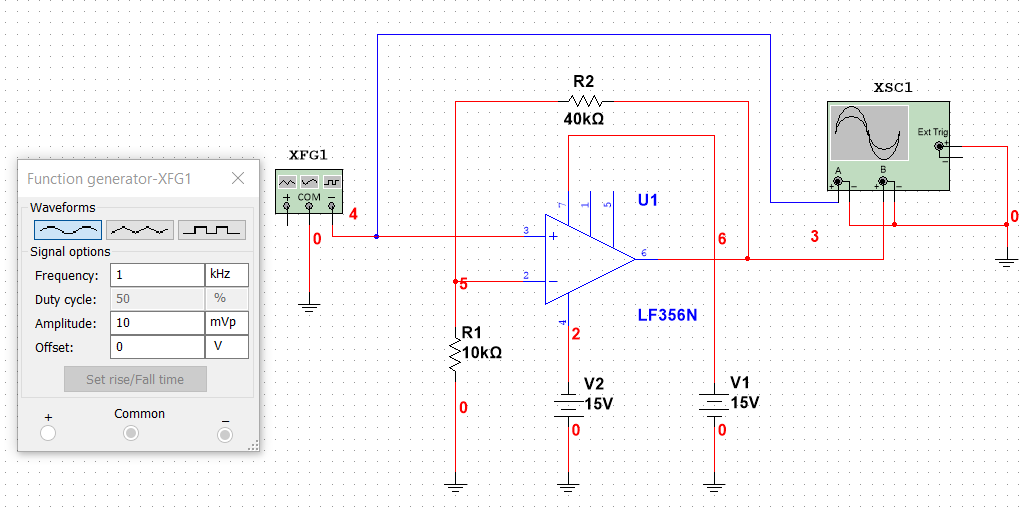
\includegraphics[width=10cm]{7}
\caption*{\textbf{Rys. 7}: Schemat układu wzmacniacza operacyjnego w układzie wzmacniacza nieodwracającego, dla którego $k_u=5$}
\end{figure}
\noindent Celem zadania było wyznaczenie wzmocnienia napięciowego przy pomocy analizy Transient. Na \textbf{Rys. 8} i \textbf{Rys. 9} widać odpowiednio ekran oscyloskopu oraz wyniki pomiarów analizy Transient. Na oscyloskopie wybrałem tryb AC by oba przebiegi były symetryczne. Łatwo zauważyć, że sygnał wyjściowy
jest nieodwrócony. Do policzenia wzmocnienia napięciowego
użyjemy wzoru $k_u=\frac{{\Delta}U_{Wy}}{{\Delta}U_{We}}$. W celu łatwych obliczeń policzę iloraz podwojonych amplitud sygnałów (dy). Z analizy Transient mam: $k_u=\frac{200.5020mV}{40.1019mV}=4.999$ zaś z obrazu oscyloskopu $k_u=\frac{2*49.832mV}{2*9.967mV}=4.999$. Wyniki są zatem zgodne.
\begin{figure}[H]
\centering

\includegraphics[width=10cm]{8}
\caption*{\textbf{Rys. 8}: Ekran oscyloskopu dla układu wzmacniacza widocznego na Rys. 7, gdzie $k_u=5$}
\end{figure}
\begin{figure}[H]
\centering
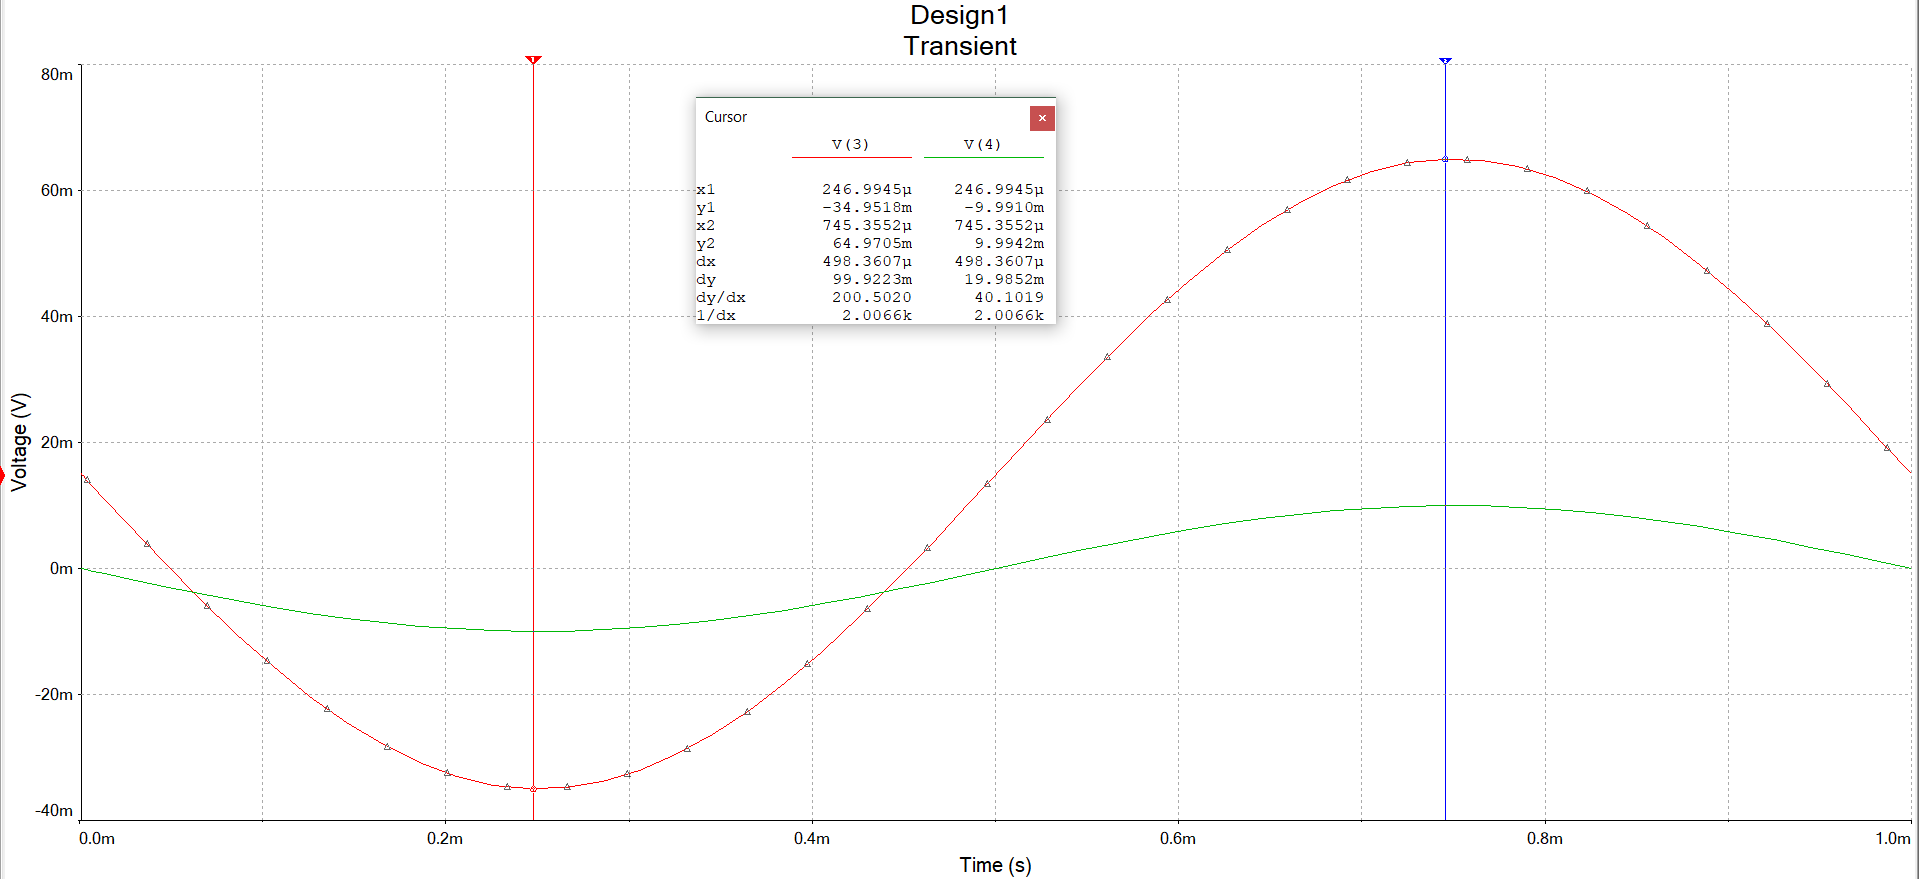
\includegraphics[width=10cm]{9}
\caption*{\textbf{Rys. 9}: Analiza Transient dla układu wzmacniacza widocznego na Rys. 7, gdzie $k_u=5$ }
\end{figure}
\subsection{Wnioski}
Wykonane ćwiczenie pokazuje, że wzór na wzmocnienie napięciowe $k_u=\frac{R_1+R_2}{R_1}$ jest poprawny i daje praktycznie dokładną wartość wzmocnienia napięciowego, co udowodniłem obliczając wzmocnienie napięciowe przy pomocy ekranu oscyloskopu i analizy Transient przy pomocy wzoru  $k_u=\frac{{\Delta}U_{Wy}}{{\Delta}U_{We}}$. W ćwiczeniu zauważyliśmy również nieodwrócony sygnał wyjściowy.
\section{Wzmacniacz operacyjny w układzie wtórnika napięciowego}
\subsection{Cel ćwiczenia}
Celem ćwiczenia było zapoznanie się z prostym układem wzmacniacza operacyjnego w układzie wtórnika napięciowego oraz wyznaczenie jego wzmocnienia napięciowego przy pomocy analizy Transient.
\subsection{Przebieg ćwiczenia}
Na pulpicie symulacyjnym zbudowałem układ wzmacniacza operacyjnego w układzie wtórnika napięciowego widoczny na \textbf{Rys. 10}. Układ zawiera dwa źródła napięcia stałego $V_1=15V$,$V_2=15V$ oraz wzmacniacz operacyjny $LF356N$. Do układu podłączyłem również generator $XFG1$, o częstotliwości $1kHz$ i amplitudzie $10mV$, oraz oscyloskop $XSC1$, które pomogły mi obserwować przebieg napięcia wejściowego i wyjściowego.
\begin{figure}[H]
\centering
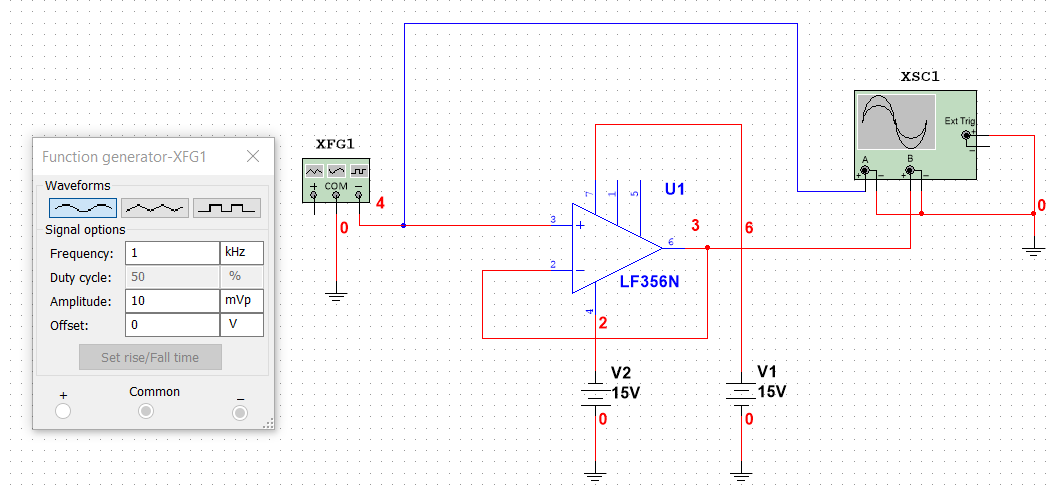
\includegraphics[width=10cm]{10}
\caption*{\textbf{Rys. 10}: Schemat układu wzmacniacza operacyjnego w układzie wtórnika napięciowego, dla którego $k_u=1$}
\end{figure}
\noindent Celem zadania było wyznaczenie wzmocnienia napięciowego przy pomocy analizy Transient. Na \textbf{Rys. 11} i \textbf{Rys. 12} widać odpowiednio ekran oscyloskopu oraz wyniki pomiarów analizy Transient. Na oscyloskopie wybrałem tryb AC by oba przebiegi były symetryczne oraz zmieniłem skale jednego z przebiegów by wykresy nie pokrywały się. Łatwo można zauważyć, że sygnał wyjściowy i sygnał wejściowy są równe - na wyjściu mamy taki sam sygnał jak na wejściu. Takie układy znajdują swoje zastosowanie w układach zawierających dzielnik napięcia. Przy zastosowaniu wzmacniacza operacyjnego z wtórnikiem 
napięcia podłączonego do wyjścia dzielnika napięciowego układ staje się zależny wyłącznie od oporów na opornikach w dzielniku napięcia. Jest tak, ponieważ na wzmacniacz nie idzie żaden prąd, nie zmienia on oporu zastępczego a jedynie kopiuje na swoje wyjście napięcie z dzielnika napięcia. Jak można się spodziewać 
wzmocnienie napięciowe $k_u=1$ co potwierdzają wyniki analizy Transient oraz ekran oscyloskopu - podwojona amplituda jest na obydwu przebiegach równa.
\begin{figure}[H]
\centering
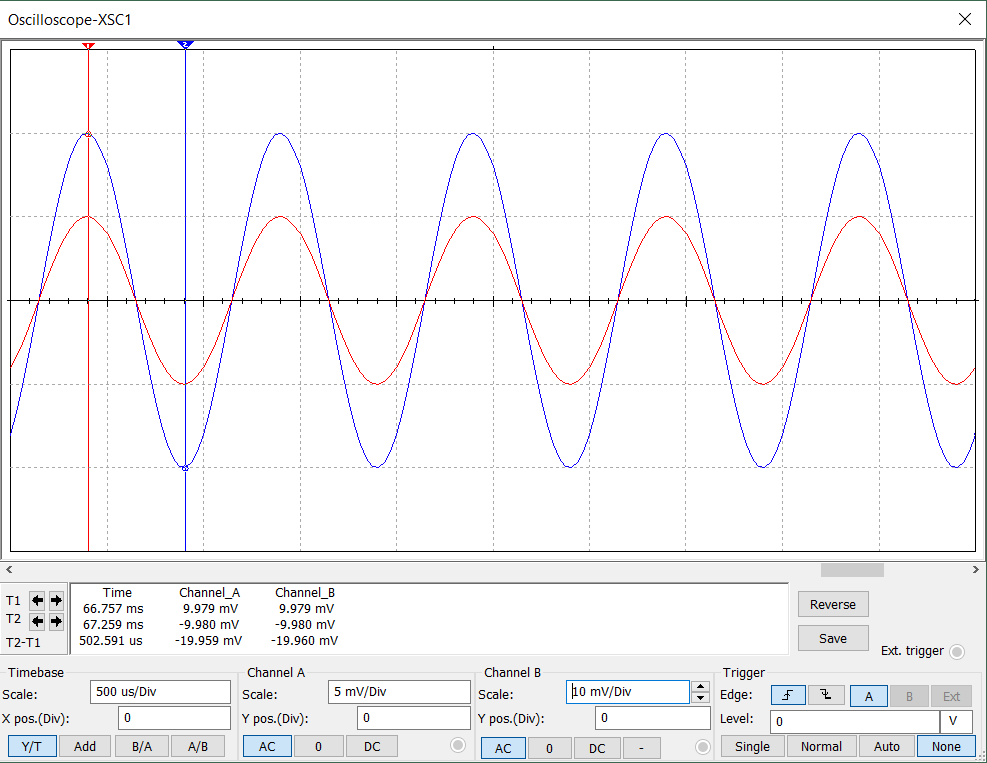
\includegraphics[width=10cm]{11}
\caption*{\textbf{Rys.11}: Ekran oscyloskopu dla układu wzmacniacza widocznego na Rys. 10, gdzie $k_u=1$}
\end{figure}
\begin{figure}[H]
\centering
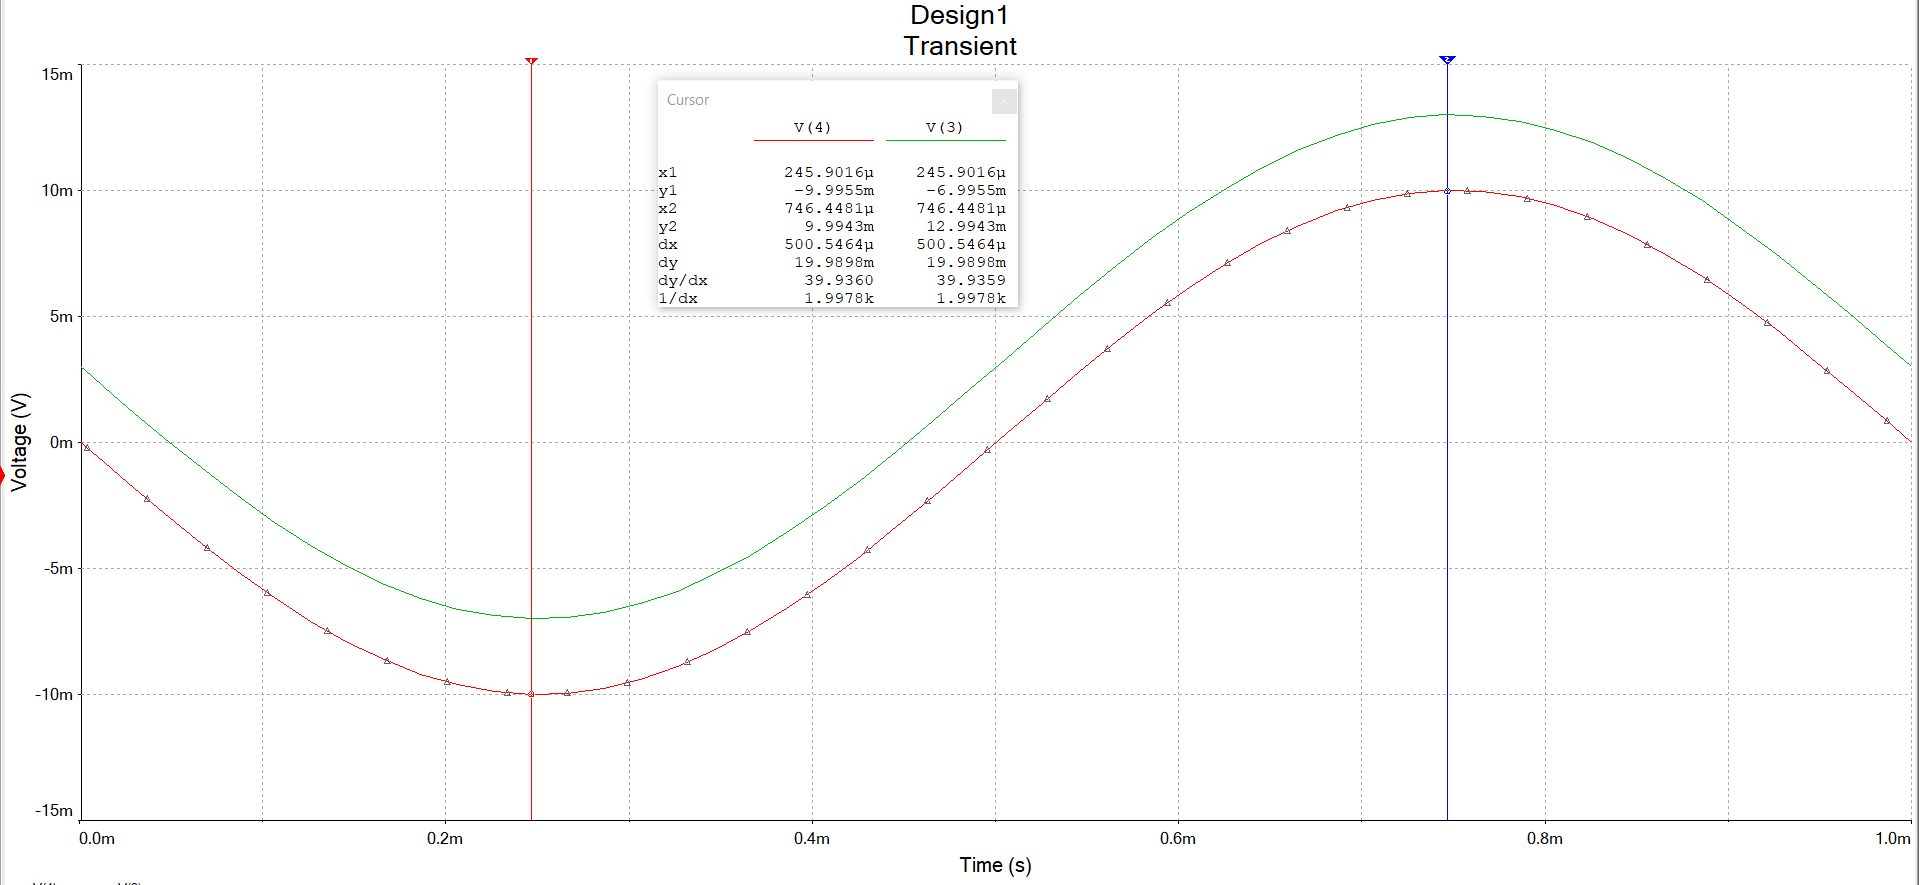
\includegraphics[width=10cm]{12}
\caption*{\textbf{Rys. 12}: Analiza Transient dla układu wzmacniacza widocznego na Rys. 10, gdzie $k_u=1$ }
\end{figure}
\subsection{Wnioski}
Wykonane ćwiczenie pokazuje, że układ wtórnika napięciowego otrzymuje na wyjściu dokładnie taki sam sygnał jak wejściowy, stąd wzmocnienie napięciowe $k_u=1$. Układ taki możemy stosować wszędzie tam, gdzie chcemy oddzielić dwie części układu tak, aby zmiany w jednej jego części nie wpływały na napięcie do niego
wpływające z jego drugiej części.
\section{Wzmacniacz operacyjny jako integrator}
\subsection{Cel ćwiczenia}
Celem ćwiczenia było zapoznanie się z prostym układem wzmacniacza operacyjnego jako integratora oraz zaobserwowanie efektu całkowania sygnału wejściowego.
\subsection{Przebieg ćwiczenia}
Na pulpicie symulacyjnym zbudowałem układ wzmacniacza operacyjnego jako integratora widoczny na \textbf{Rys. 13}. Układ zawiera dwa źródła napięcia stałego $V_1=15V$,$V_2=15V$, dwa rezystory $R_1=10k\Omega$,$R_2=100k\Omega$, kondensator $C_1=6.8nF$ oraz wzmacniacz operacyjny $LF356N$. Do układu podłączyłem również generator $XFG1$ (sygnał prostokątny), o częstotliwości $10kHz$, wypełnieniu $30\%$, amplitudzie $10mV$, oraz oscyloskop $XSC1$, które pomogły mi obserwować przebieg napięcia wejściowego i wyjściowego.
\begin{figure}[H]
\centering
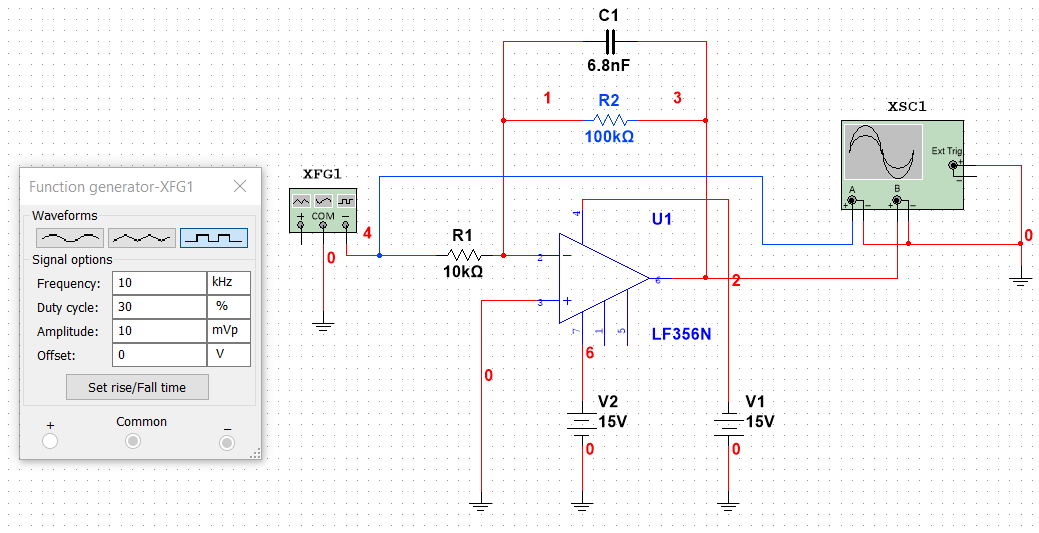
\includegraphics[width=10cm]{13}
\caption*{\textbf{Rys. 13}: Schemat układu wzmacniacza operacyjnego jako integratora}
\end{figure}
\noindent Celem zadania było zaobserwowanie efektu całkowania sygnału wejściowego w układzie widocznym na \textbf{Rys. 13}. Na \textbf{Rys. 14} widać ekran oscyloskopu. Widać na nim efekt całkowania sygnału wejściowego (przebieg w kolorze niebieskim). Napięcie wyjściowe dane jest wzorem: 
$U_{Wy}=\frac{-1}{C}{\int}i(t)dt=\frac{-1}{R_1*C}{\int}U_{We}(t)dt$.
\begin{figure}[H]
\centering
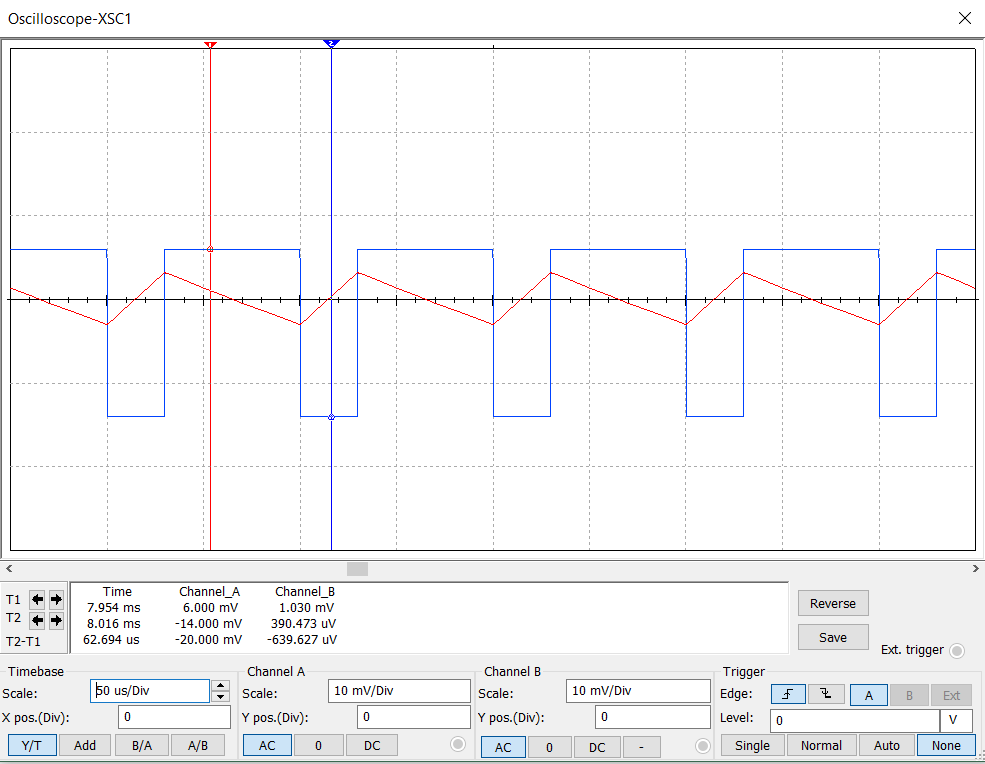
\includegraphics[width=10cm]{14}
\caption*{\textbf{Rys. 14}: Ekran oscyloskopu dla układu wzmacniacza widocznego na Rys. 13. Sygnał wejściowy jest zaznaczony kolorem niebieskim zaś wyjściowy czerwonym. }
\end{figure}
\subsection{Wnioski}
Wykonane ćwiczenie pokazuje, że układ wzmacniacza operacyjnego jako integratora skutecznie wykonuje całkowanie sygnału wejściowego zgodnie ze wzorem $U_{Wy}=\frac{-1}{C}{\int}i(t)dt=\frac{-1}{R_1*C}{\int}U_{We}(t)dt$. 
\section{Wzmacniacz operacyjny jako aktywny detektor szczytowy}
\subsection{Cel ćwiczenia}
Celem ćwiczenia było zapoznanie się z prostym układem wzmacniacza operacyjnego jako aktywnego detektora szczytowego oraz zaobserwowanie sygnału wejściowego i wyjściowego.
\subsection{Przebieg ćwiczenia}
Na pulpicie symulacyjnym zbudowałem układ wzmacniacza operacyjnego jako aktywnego detektora szczytowego widoczny na \textbf{Rys. 15}. Układ zawiera dwa źródła napięcia stałego $V_1=15V$,$V_2=15V$, trzy rezystory $R_1=1k\Omega$,$R_2=1k\Omega$,$R_3=1k\Omega$, kondensator $C_1=1{\mu}F$, diodę 
$BAV19$, tranzystor $IRF540$ oraz wzmacniacz operacyjny $LM715CH$. Do układu podłączyłem również trzy generatory $XFG1$,$XFG2$,$XFG3$, których parametry widać na \textbf{Rys. 16}, oraz oscyloskop $XSC1$.
\begin{figure}[H]
\centering
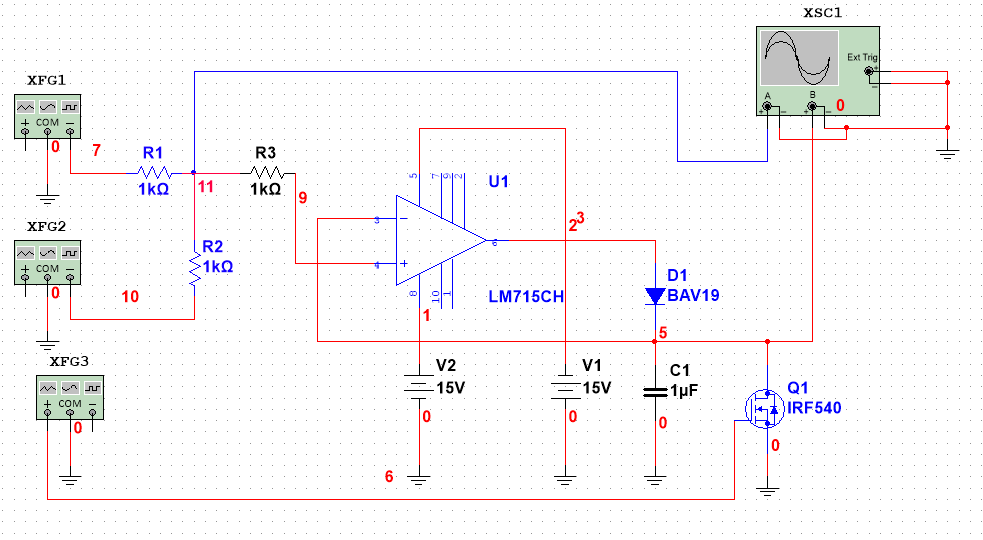
\includegraphics[width=10cm]{15}
\caption*{\textbf{Rys. 15}: Schemat układu wzmacniacza operacyjnego jako aktywnego detektora szczytowego}
\end{figure}
\begin{figure}[H]
\centering
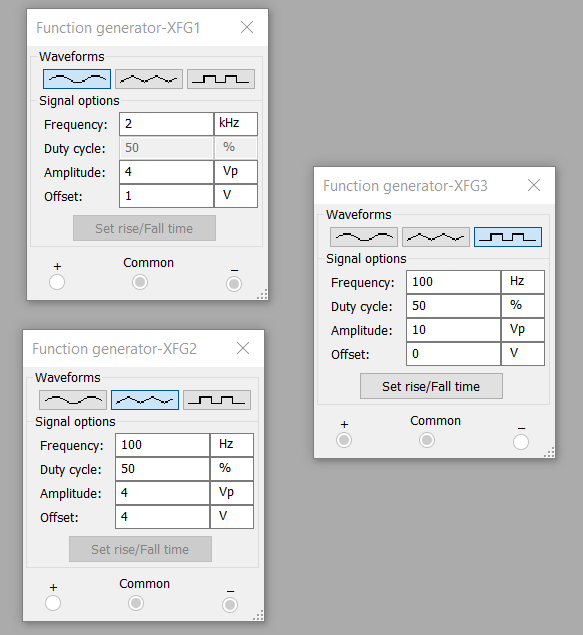
\includegraphics[width=5cm]{16}
\caption*{\textbf{Rys. 16}: Parametry generatorów podłączonych do układu z Rys. 15 }
\end{figure}
\noindent Generatory $XFG1$ i $XFG2$ podają na wejście nieodwracające wzmacniacza sygnał wejściowy będący złożeniem sygnału sinusoidalnego oraz trójkątnego. Generator $XFG3$ podaje zaś impuls zerujący do tranzystora, który resetuje sygnał wyjściowy po osiągnięciu przez niego wartości maksymalnej. Działanie układu
widać na \textbf{Rys. 17}. Na rysunku bardzo dobrze widać to, że sygnał wyjściowy jest największą do tej pory wartością sygnału wejściowego.
\begin{figure}[H]
\centering
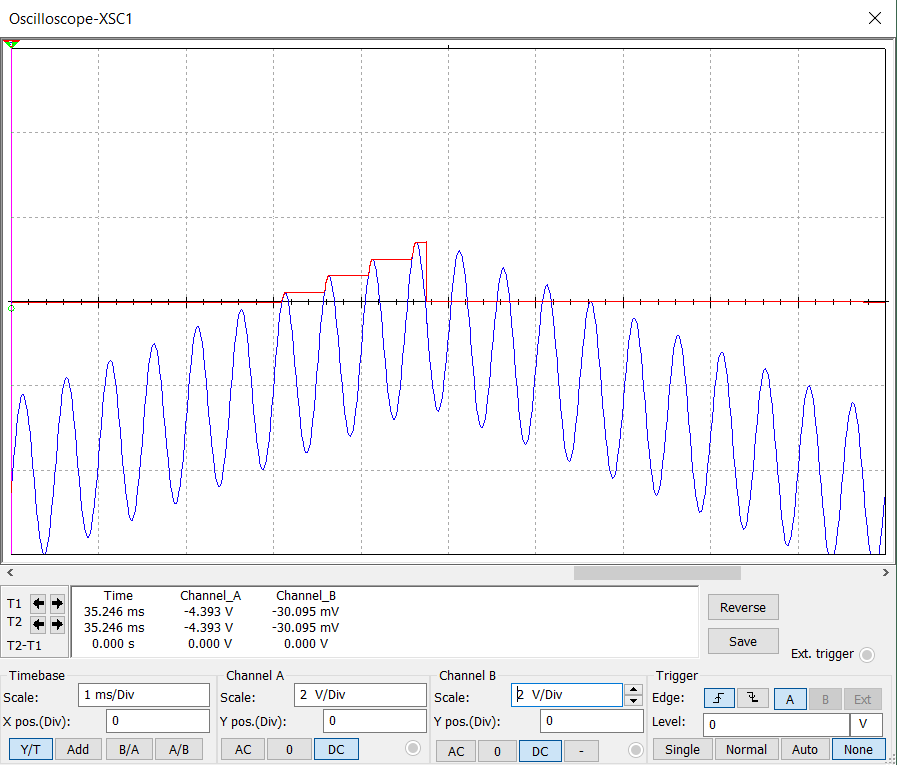
\includegraphics[width=10cm]{17}
\caption*{\textbf{Rys. 17}: Ekran oscyloskopu dla układu wzmacniacza widocznego na Rys. 15. Sygnał wejściowy jest zaznaczony kolorem niebieskim, zaś wyjściowy czerwonym. }
\end{figure}
\subsection{Wnioski}
Wykonane ćwiczenie pokazuje, że układ wzmacniacza operacyjnego jako aktywnego detektora szczytowego działa poprawnie, a sygnał wyjściowy do momentu wyzerowania jest największą do tej pory wartością sygnału wejściowego.
\section{Wzmacniacz operacyjny jako detektor progowy z histerezą}
\subsection{Cel ćwiczenia}
Celem ćwiczenia było zapoznanie się z prostym układem wzmacniacza operacyjnego jako detektora progowego z histerezą oraz obliczenie oporu i zaobserwowanie sygnału wejściowego i wyjściowego.
\subsection{Przebieg ćwiczenia}
Na pulpicie symulacyjnym zbudowałem układ wzmacniacza operacyjnego jako detektora progowego z histerezą widoczny na \textbf{Rys. 18}. Układ zawiera dwa źródła napięcia stałego $V_1=15V$,$V_2=15V$, trzy rezystory $R_1=10k\Omega$,$R_2$,$R_3=10k\Omega$ oraz wzmacniacz operacyjny $LM715CH$. Wartość 
oporu $R_2$ należało policzyć na podstawie wzorów $U_{P1}=\frac{R_1}{R_1+R_2}*U_{Z+}$ oraz $U_{P2}=\frac{R_1}{R_1+R_2}*U_{Z-}$ wiedząc, że $U_{P1}=2V$,$U_{P2}=-2V$, $U_{Z+}=15V$,$U_{Z-}=-15V$. Po przekształceniu wzorów i podstawieniu odpowiednich wartości otrzymałem $R_2=65k\Omega$.
Do układu podłączyłem również generator $XFG1$, o częstotliwości $50Hz$ i amplitudzie $5V$ oraz oscyloskop $XSC1$.
\begin{figure}[H]
\centering
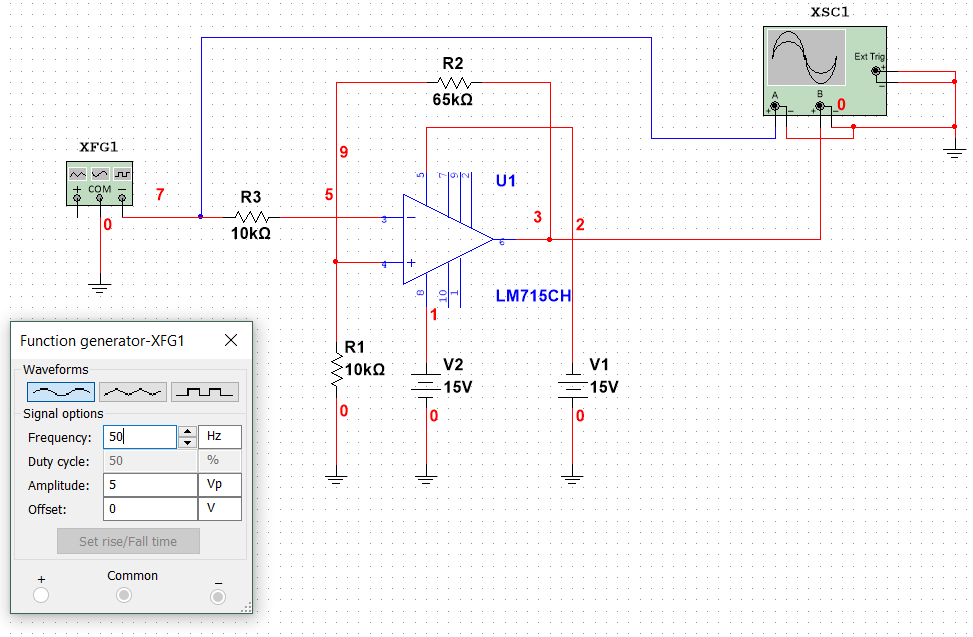
\includegraphics[width=10cm]{18}
\caption*{\textbf{Rys. 18}: Schemat układu wzmacniacza operacyjnego jako detektora progowego z histerezą, gdzie $U_{P1}=2V$, $U_{P2}=-2V$}
\end{figure}
\noindent Celem zadania było znalezienie wartości $U_{P1}$,$U_{P2}$ w obwodzie i sprawdzenie czy są one bliskie wartościom przez nas narzuconym ($2V$ i $-2V$). Na \textbf{Rys. 19} i \textbf{Rys. 20} widać ekran oscyloskopu w trybie odpowiednio Y/T oraz B/A. W trybie Y/T znajdujemy nasze wartości znajdując punkty przecięcia 
sygnału wejściowego i wyjściowego. W naszym przypadku zmierzone wartości to $U_{P1}=1.760V$ oraz $U_{P2}=-1.747V$. W trybie B/A znajdujemy nasze wartości punktów, w których wartość zmienia się z $U_{Z-}$ na $U_{Z+}$ oraz z $U_{Z+}$ na $U_{Z-}$. W naszym przypadku są to $U_{P1}=1.759V$ oraz 
$U_{P2}=-1.740V$. Na koniec w taki sam sposób jak w trybie Y/T zmierzyłem wartości używając analizy Transient (\textbf{Rys. 21}). Zmierzone wartości to $U_{P1}=1.7190V$ oraz $U_{P2}=-1.6869V$. 
\begin{figure}[H]
\centering
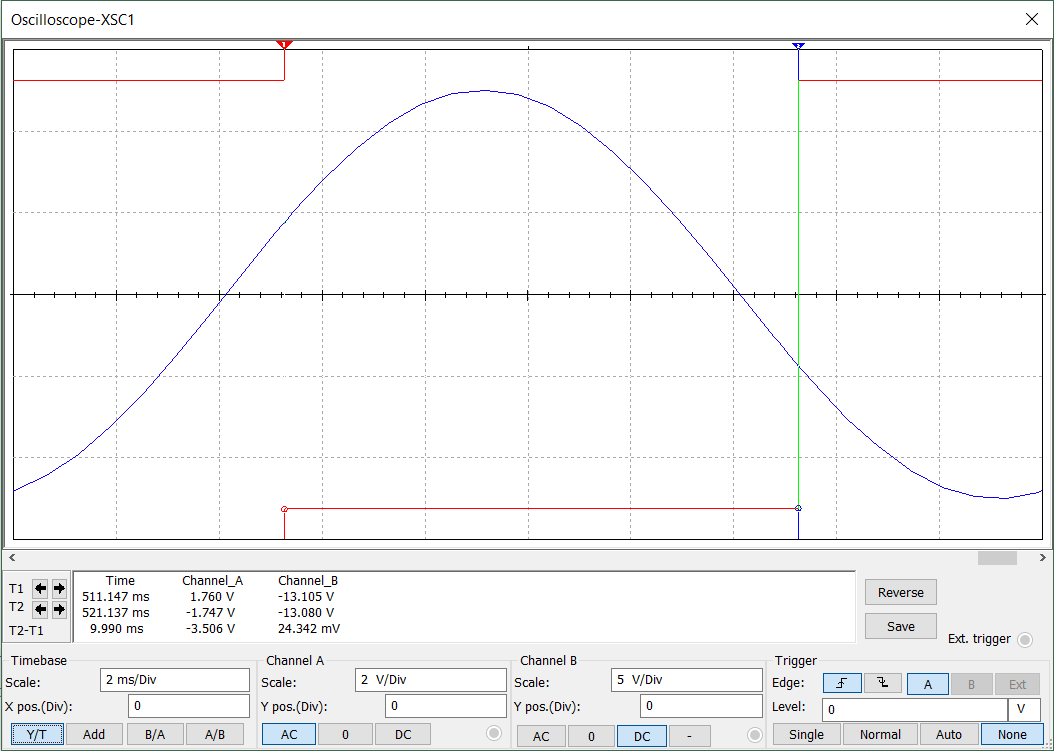
\includegraphics[width=10cm]{19}
\caption*{\textbf{Rys. 19}: Ekran oscyloskopu obwodu z Rys. 18 w trybie Y/T}
\end{figure}
\begin{figure}[H]
\centering
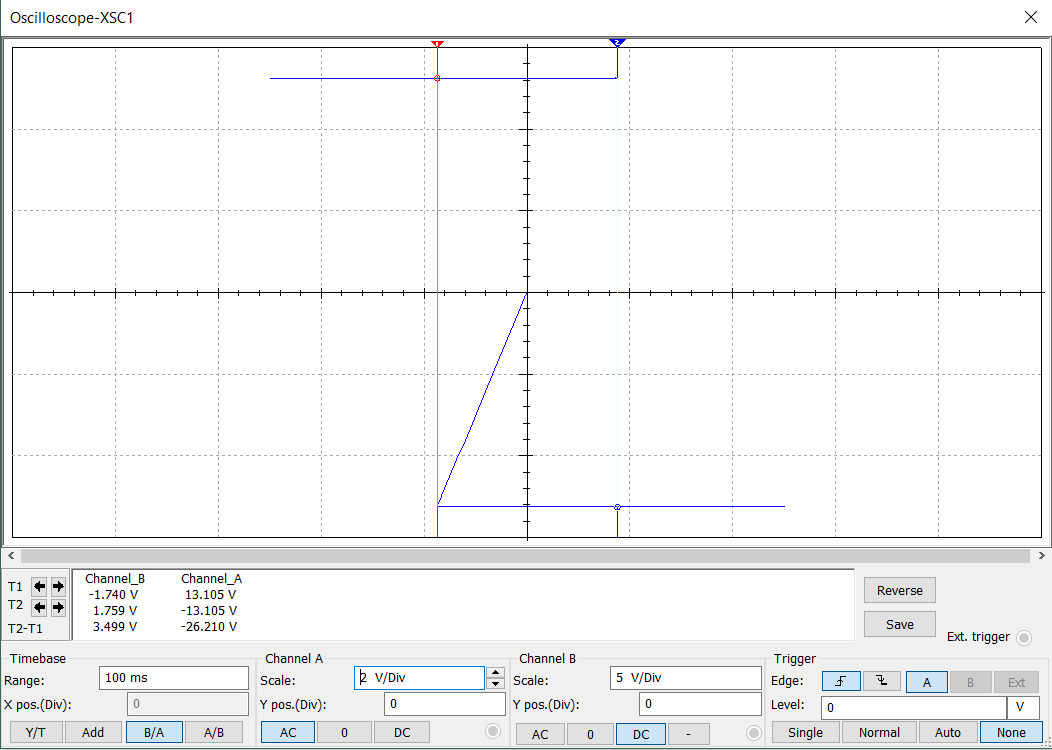
\includegraphics[width=10cm]{20}
\caption*{\textbf{Rys. 20}: Ekran oscyloskopu obwodu z Rys. 18 w trybie B/A}
\end{figure}
\begin{figure}[H]
\centering
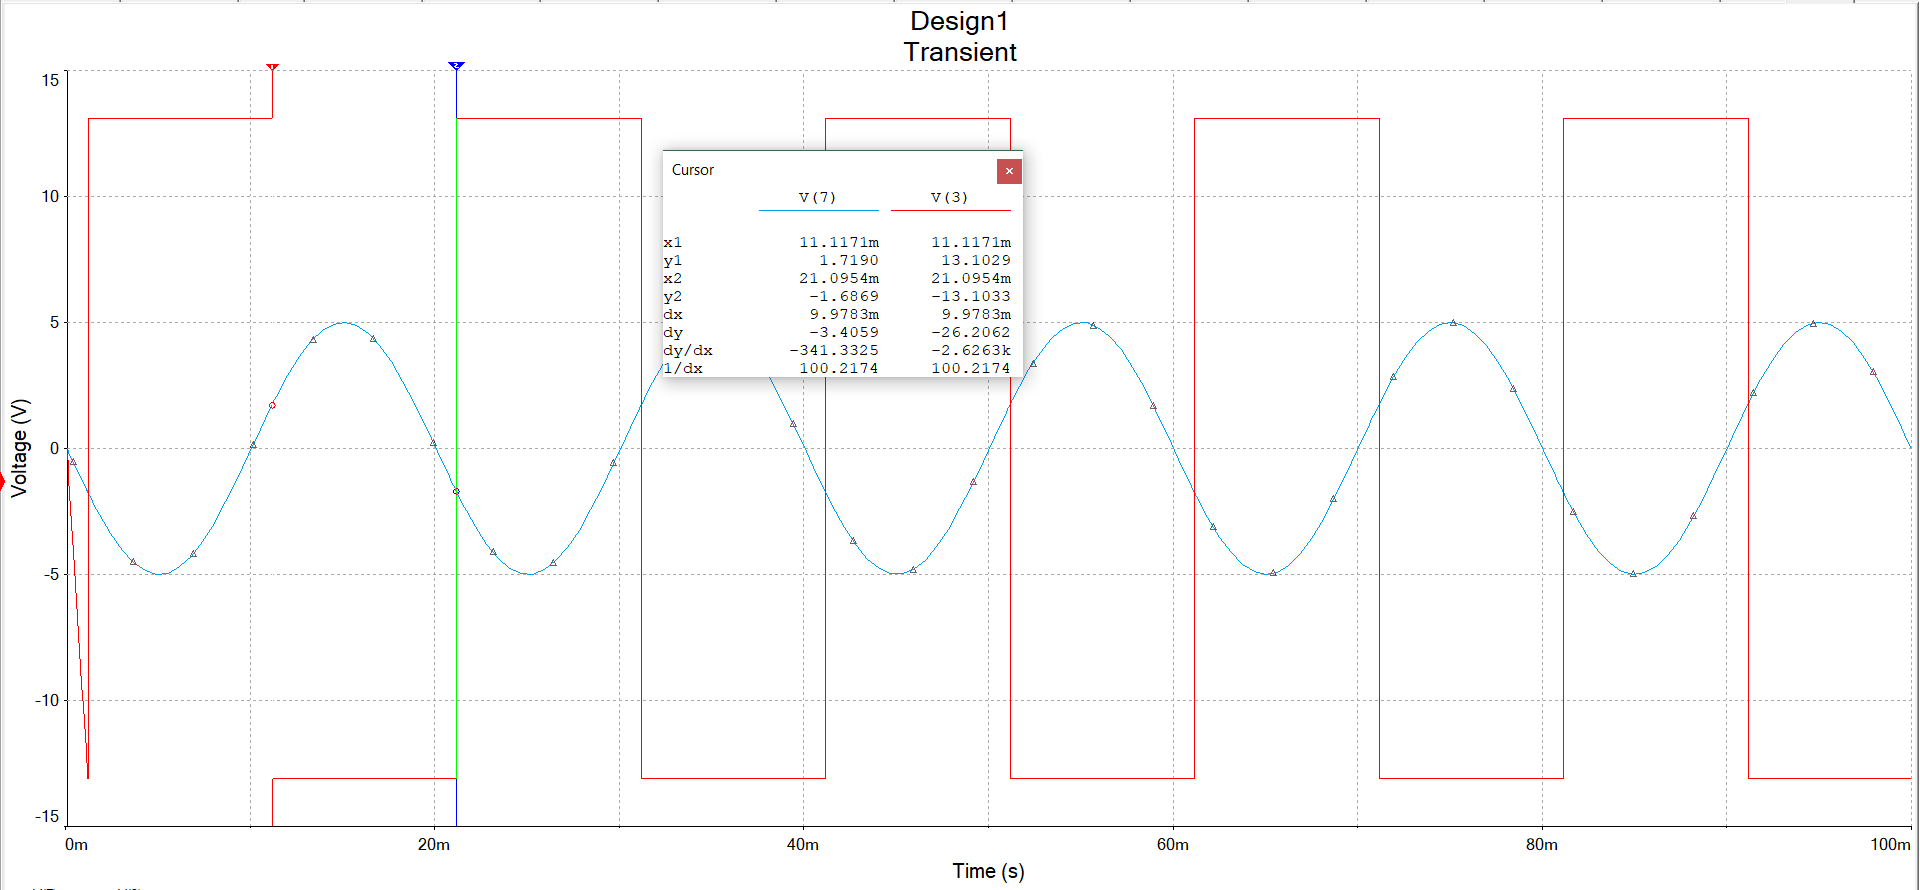
\includegraphics[width=12cm]{21}
\caption*{\textbf{Rys. 21}: Analiza Transient dla obwodu z Rys. 18}
\end{figure}
Zmierzone wartości pokazane są w tabeli na \textbf{Rys. 22}.
\begin{figure}[H]
\centering
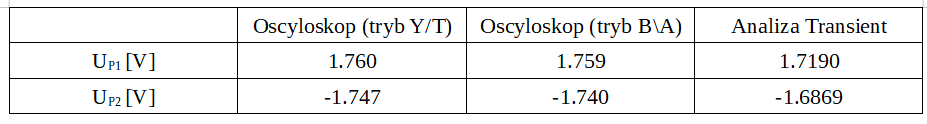
\includegraphics[width=10cm]{22}
\caption*{\textbf{Rys. 22}: Tabela z wszystkimi wynikami pomiarów ćwiczenia}
\end{figure}
\subsection{Wnioski}
Wykonane ćwiczenie pokazuje, że uklad wzmacniacza operacyjnego jako detektora progowego z histerezą jest poprawny, lecz niestabilny. Napięcia przełączania były nieco mniejsze niż zadane, co prawdopodobnie było skutkiem nieosiągania odpowiedniej wartości napięć $U_{Z+}$ i $U_{Z-}$ (około $13.1V$).
\section{Wzmacniacz operacyjny w układzie wzmacniacza różnicowego}
\subsection{Cel ćwiczenia}
Celem ćwiczenia było zapoznanie się z prostym układem wzmacniacza operacyjnego w układzie wzmacniacza różnicowego oraz zaobserwowanie sygnału wyjściowego jako różnicy dwóch sygnałów wejściowych.
\subsection{Przebieg ćwiczenia}
Na pulpicie symulacyjnym zbudowałem układ wzmacniacza operacyjnego w układzie wzmacniacza różnicowego widoczny na \textbf{Rys. 23}. Układ zawiera dwa źródła napięcia stałego $V_1=15V$,$V_2=15V$, cztery rezystory $R_1=1k\Omega$,$R_2=1k\Omega$,$R_3=1k\Omega$,$R_4=1k\Omega$ oraz wzmacniacz operacyjny $LF356N$ Do układu podłączyłem również dwa generatory $XFG1$ (sygnał sinusoidalny) oraz $XFG2$ (sygnał prostokątny) oraz oscyloskop $XSC1$. Generator $XFG1$ ma częstotliwość $5kHz$ oraz amplitudę $50mV$, zaś generator $XFG2$ ma częstotliwość $500Hz$, wypełnienie $50\%$ i amplitudę $500mV$. Jeden sygnał ma dużą częstotliwość i małą amplitudę, drugi zaś małą częstotliwość i dużą amplitudę.
\begin{figure}[H]
\centering
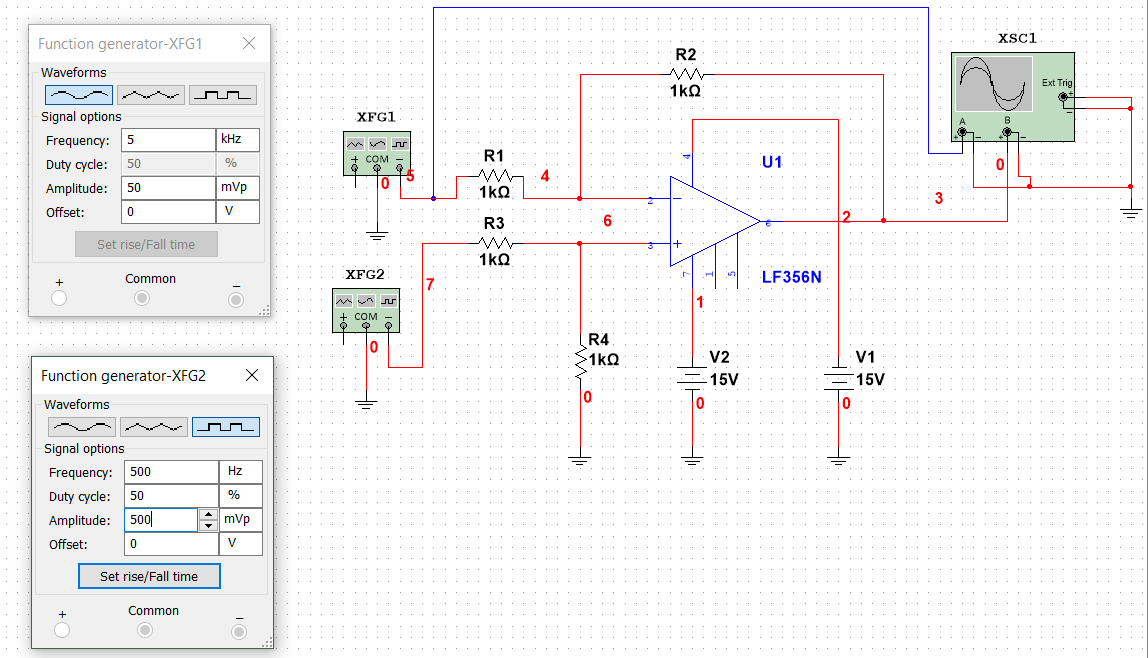
\includegraphics[width=10cm]{23}
\caption*{\textbf{Rys. 23}: Schemat układu wzmacniacza operacyjnego w układzie wzmacniacza różnicowego z sygnałami wejściowymi sinusoidalnym i prostokątnym}
\end{figure}
\noindent Sygnał wyjściowy dany jest wzorem $u_{Wy}=\frac{R2}{R1}*(u_{we+}-u_{we-})$, gdzie $u_{we+}$ to napięcie na wejściu nieodwracającym, zaś $u_{we-}$ to napięcie na wejściu odwracającym. Na \textbf{Rys. 24} widać sygnał wyjściowy czyli efekt różnicy dwóch sygnałów wejściowych. Na \textbf{Rys. 25} widać sygnał wyjściowy przy innych parametrach sygnałów wejściowych, które widać na owym rysunku.
\begin{figure}[H]
\centering
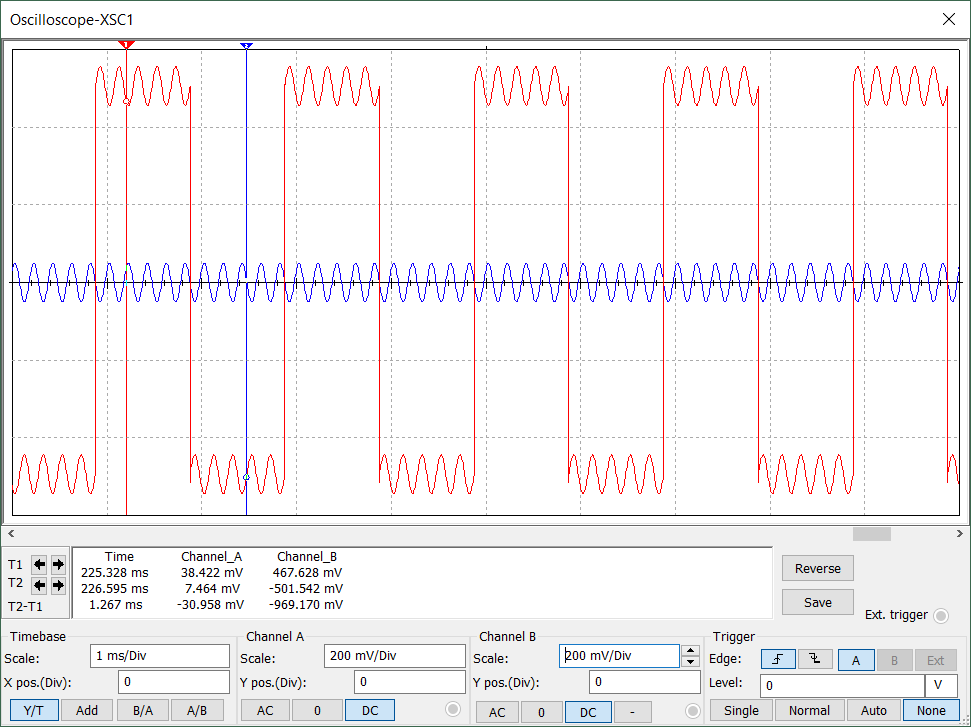
\includegraphics[width=10cm]{24}
\caption*{\textbf{Rys. 24}: Ekran oscyloskopu dla układu z Rys. 23}
\end{figure}
\begin{figure}[H]
\centering
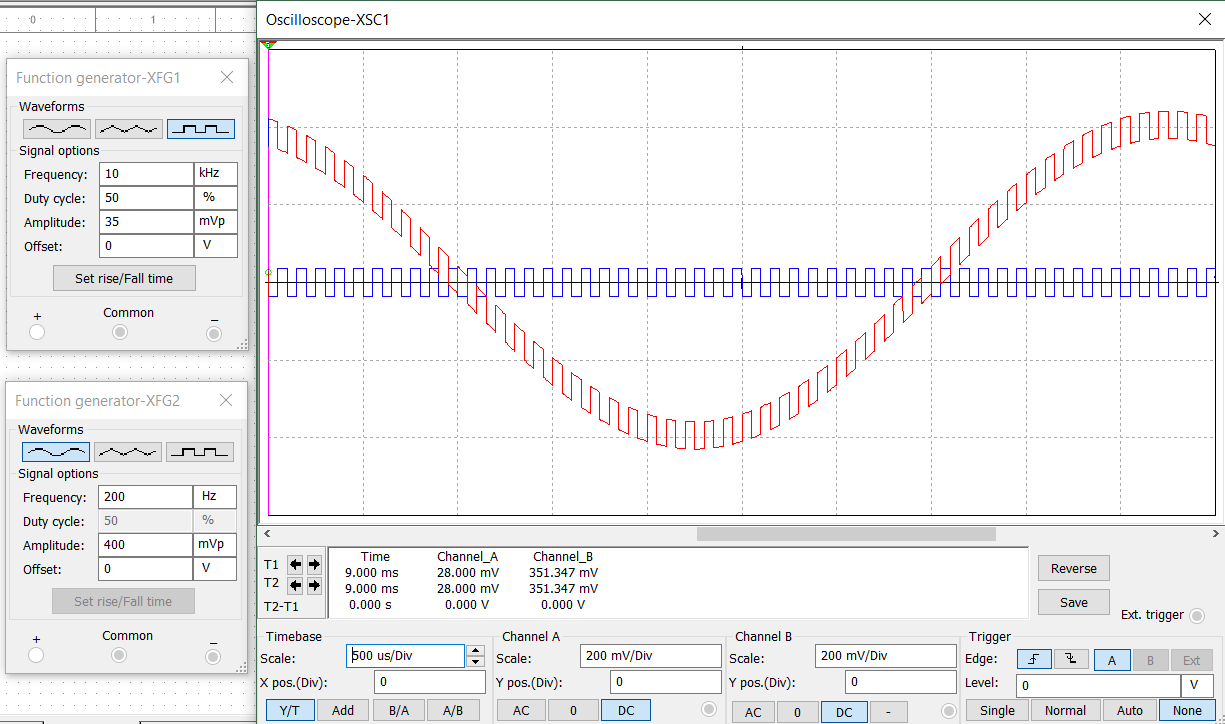
\includegraphics[width=10cm]{25}
\caption*{\textbf{Rys. 25}: Ekran oscyloskopu dla układu z Rys. 23 ze zmienionymi parametrami wejściowymi}
\end{figure}
\subsection{Wnioski}
Wykonane ćwiczenie pokazuje, że układ wzmacniacza operacyjnego w układzie wzmacniacza różnicowego działa poprawnie. Sygnał wyjściowy jest różnicą dwóch sygnałów wejściowych.
\end{document}